\documentclass[preview]{standalone} 

\usepackage{tikz} 

\begin{document} 
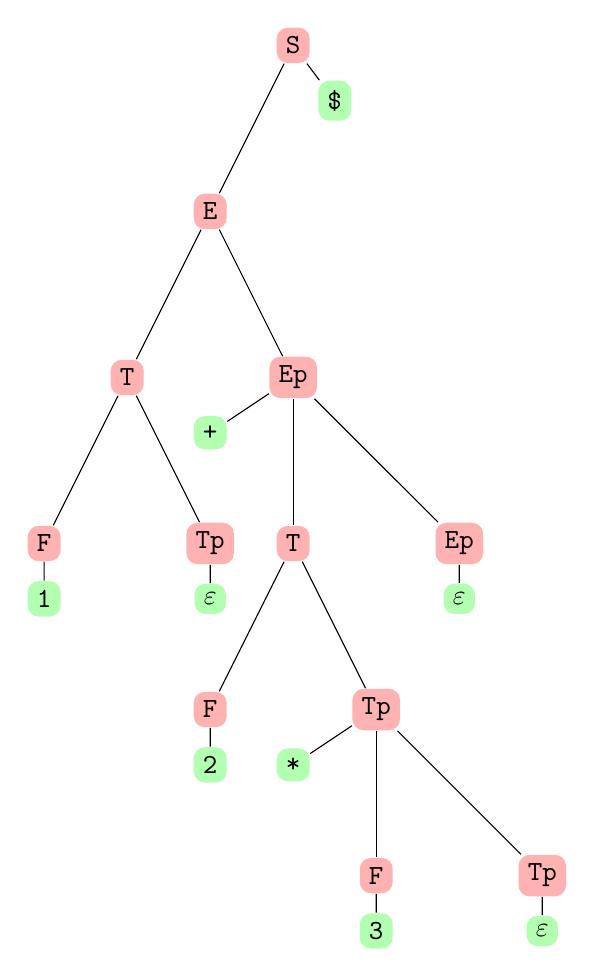
\begin{tikzpicture}[level distance=6em, every node/.style={fill=red!30,rounded corners,font=\ttfamily}]

\node{S}
child[sibling distance=6em]{
node{E}child[sibling distance=6em]{
node{T}child[sibling distance=6em]{
node{F}child[level distance=2em, sibling distance=3em]{node[fill=green!30,rounded corners,font=\ttfamily]{1}}
}
child[sibling distance=6em]{
node{Tp}child[level distance=2em, sibling distance=3em]{node[fill=green!30,rounded corners,font=\ttfamily]{$\varepsilon$}}
}
}
child[sibling distance=6em]{
node{Ep}child[level distance=2em, sibling distance=3em]{node[fill=green!30,rounded corners,font=\ttfamily]{+}}
child[sibling distance=6em]{
node{T}child[sibling distance=6em]{
node{F}child[level distance=2em, sibling distance=3em]{node[fill=green!30,rounded corners,font=\ttfamily]{2}}
}
child[sibling distance=6em]{
node{Tp}child[level distance=2em, sibling distance=3em]{node[fill=green!30,rounded corners,font=\ttfamily]{*}}
child[sibling distance=6em]{
node{F}child[level distance=2em, sibling distance=3em]{node[fill=green!30,rounded corners,font=\ttfamily]{3}}
}
child[sibling distance=6em]{
node{Tp}child[level distance=2em, sibling distance=3em]{node[fill=green!30,rounded corners,font=\ttfamily]{$\varepsilon$}}
}
}
}
child[sibling distance=6em]{
node{Ep}child[level distance=2em, sibling distance=3em]{node[fill=green!30,rounded corners,font=\ttfamily]{$\varepsilon$}}
}
}
}
child[level distance=2em, sibling distance=3em]{node[fill=green!30,rounded corners,font=\ttfamily]{\$}}
;
\end{tikzpicture}
\end{document}
